\documentclass[ngerman]{beamer}
\usepackage[T1]{fontenc}
\usepackage[utf8]{inputenc}
\usepackage{babel}
\usepackage{listings}
\usepackage{csquotes}
\usepackage{amsmath}
\usepackage{hyperref}

\usetheme{Darmstadt}


\lstset{
    basicstyle=\tiny\ttfamily,
    frame=single
}


\subject{Projektpräsentation}

\title{Correlation Power Analysis on the ChaCha Cipher}

\subtitle{Analyse, Implementierung \& Auswertung}

\author{Jonathan Klamroth}

\date{Sommersemester 2020}




\begin{document}



\begin{frame}

    \maketitle

\end{frame}



\section{Projekt}

\begin{frame}

    \frametitle{Aufgabe}


    \begin{itemize}
        \item CPA Angriff auf ChaCha oder Salsa20 $\rightarrow$ ChaCha
        \item Basierend auf einem von zwei Papern $\rightarrow$ ``Don't fall
            into a trap: Physical side-channel analysis of ChaCha20-Poly1305''
        \item Hardware \& Software Aufbau darstellen
    \end{itemize}

\end{frame}



\section{ChaCha}

\begin{frame}

    \frametitle{Allgemeines}


    \begin{itemize}
        \item spezifiziert im RFC 7539
        \item Verwendung in TLSv1.3
        \item Stromchiffre
        \item ARX-Chiffre
        \item basiert auf Salsa20
        \item 256-bit Schlüssel, 512-bit Blocklänge, 32-bit Counter, 96-bit
            Nonce
    \end{itemize}

\end{frame}



\begin{frame}

    \frametitle{Algorithmus}


    \begin{itemize}
        \item Zustand bestehend aus 16 32-bit Wörtern
        \item Initialzustand aus Konstanten, Schlüssel, Counter und Nonce
        \item 20 Runden
        \item vier ``quarterround''s pro Runde
        \item abwechselnd vertikal und diagonal
        \item Initialzustand am Ende addieren
    \end{itemize}

\end{frame}



\begin{frame}[fragile]

    \frametitle{Initialzustand}


    \begin{lstlisting}
v0  = C0        v1  = C1        v2  = C2        v3  = C3
v4  = k0        v5  = k1        v6  = k2        v7  = k3
v8  = k4        v9  = k5        v10 = k6        v11 = k7
v12 = counter   v13 = nonce0    v14 = nonce1    v15 = nonce2

C0 = 0x61707865         # 'expa'
C1 = 0x3320646e         # 'nd 3'
C2 = 0x79622d32         # '2-by'
C3 = 0x6b206574         # 'te k'
    \end{lstlisting}


\end{frame}



\begin{frame}[fragile]

    \frametitle{Doppelrunde}


    \begin{lstlisting}[]
v0',  v4',  v8',  v12' = quarterround(v0,  v4,  v8,  v12)
v1',  v5',  v9',  v13' = quarterround(v1,  v5,  v9,  v13)
v2',  v6',  v10', v14' = quarterround(v2,  v6,  v10, v14)
v3',  v7',  v11', v15' = quarterround(v3,  v7,  v11, v15)

v0'',  v5'',  v10'', v15'' = quarterround(v0',  v5',  v10', v15')
v1'',  v6'',  v11'', v12'' = quarterround(v1',  v6',  v11', v12')
v2'',  v7'',  v8'',  v13'' = quarterround(v2',  v7',  v8',  v13')
v3'',  v4'',  v9'',  v14'' = quarterround(v3',  v4',  v9',  v14')
    \end{lstlisting}


\end{frame}



\begin{frame}[fragile]

    \frametitle{quarterround}


    \begin{lstlisting}[]
Alle Variablen sind 32-bit Woerter!
x << n := rotate_left(x, n)

Parameter: a0, b0, c0, d0

a1 = a0 + b0    d1 = d0 ^ a1    d2 = d1 << 16
c1 = c0 + d2    b1 = b0 ^ c1    b2 = b1 << 12
a2 = a1 + b2    d3 = d2 ^ a2    d4 = d3 << 8
c2 = c1 + d2    b3 = b2 ^ c2    b4 = b3 << 7

return a2, b4, c2, d4
    \end{lstlisting}


\end{frame}



\section{Angriff}

\begin{frame}

    \frametitle{Ansatz}


    \begin{itemize}
        \item zwei Varianten: volle/reduzierte Kontrolle
        \item die erste bzw. die ersten beiden Runden angreifen
        \item Key direkt bzw. indirekt über Zwischenzustand wiederherstellen
    \end{itemize}

\end{frame}



\begin{frame}

    \frametitle{Hardware-Aufbau}


    \centering
    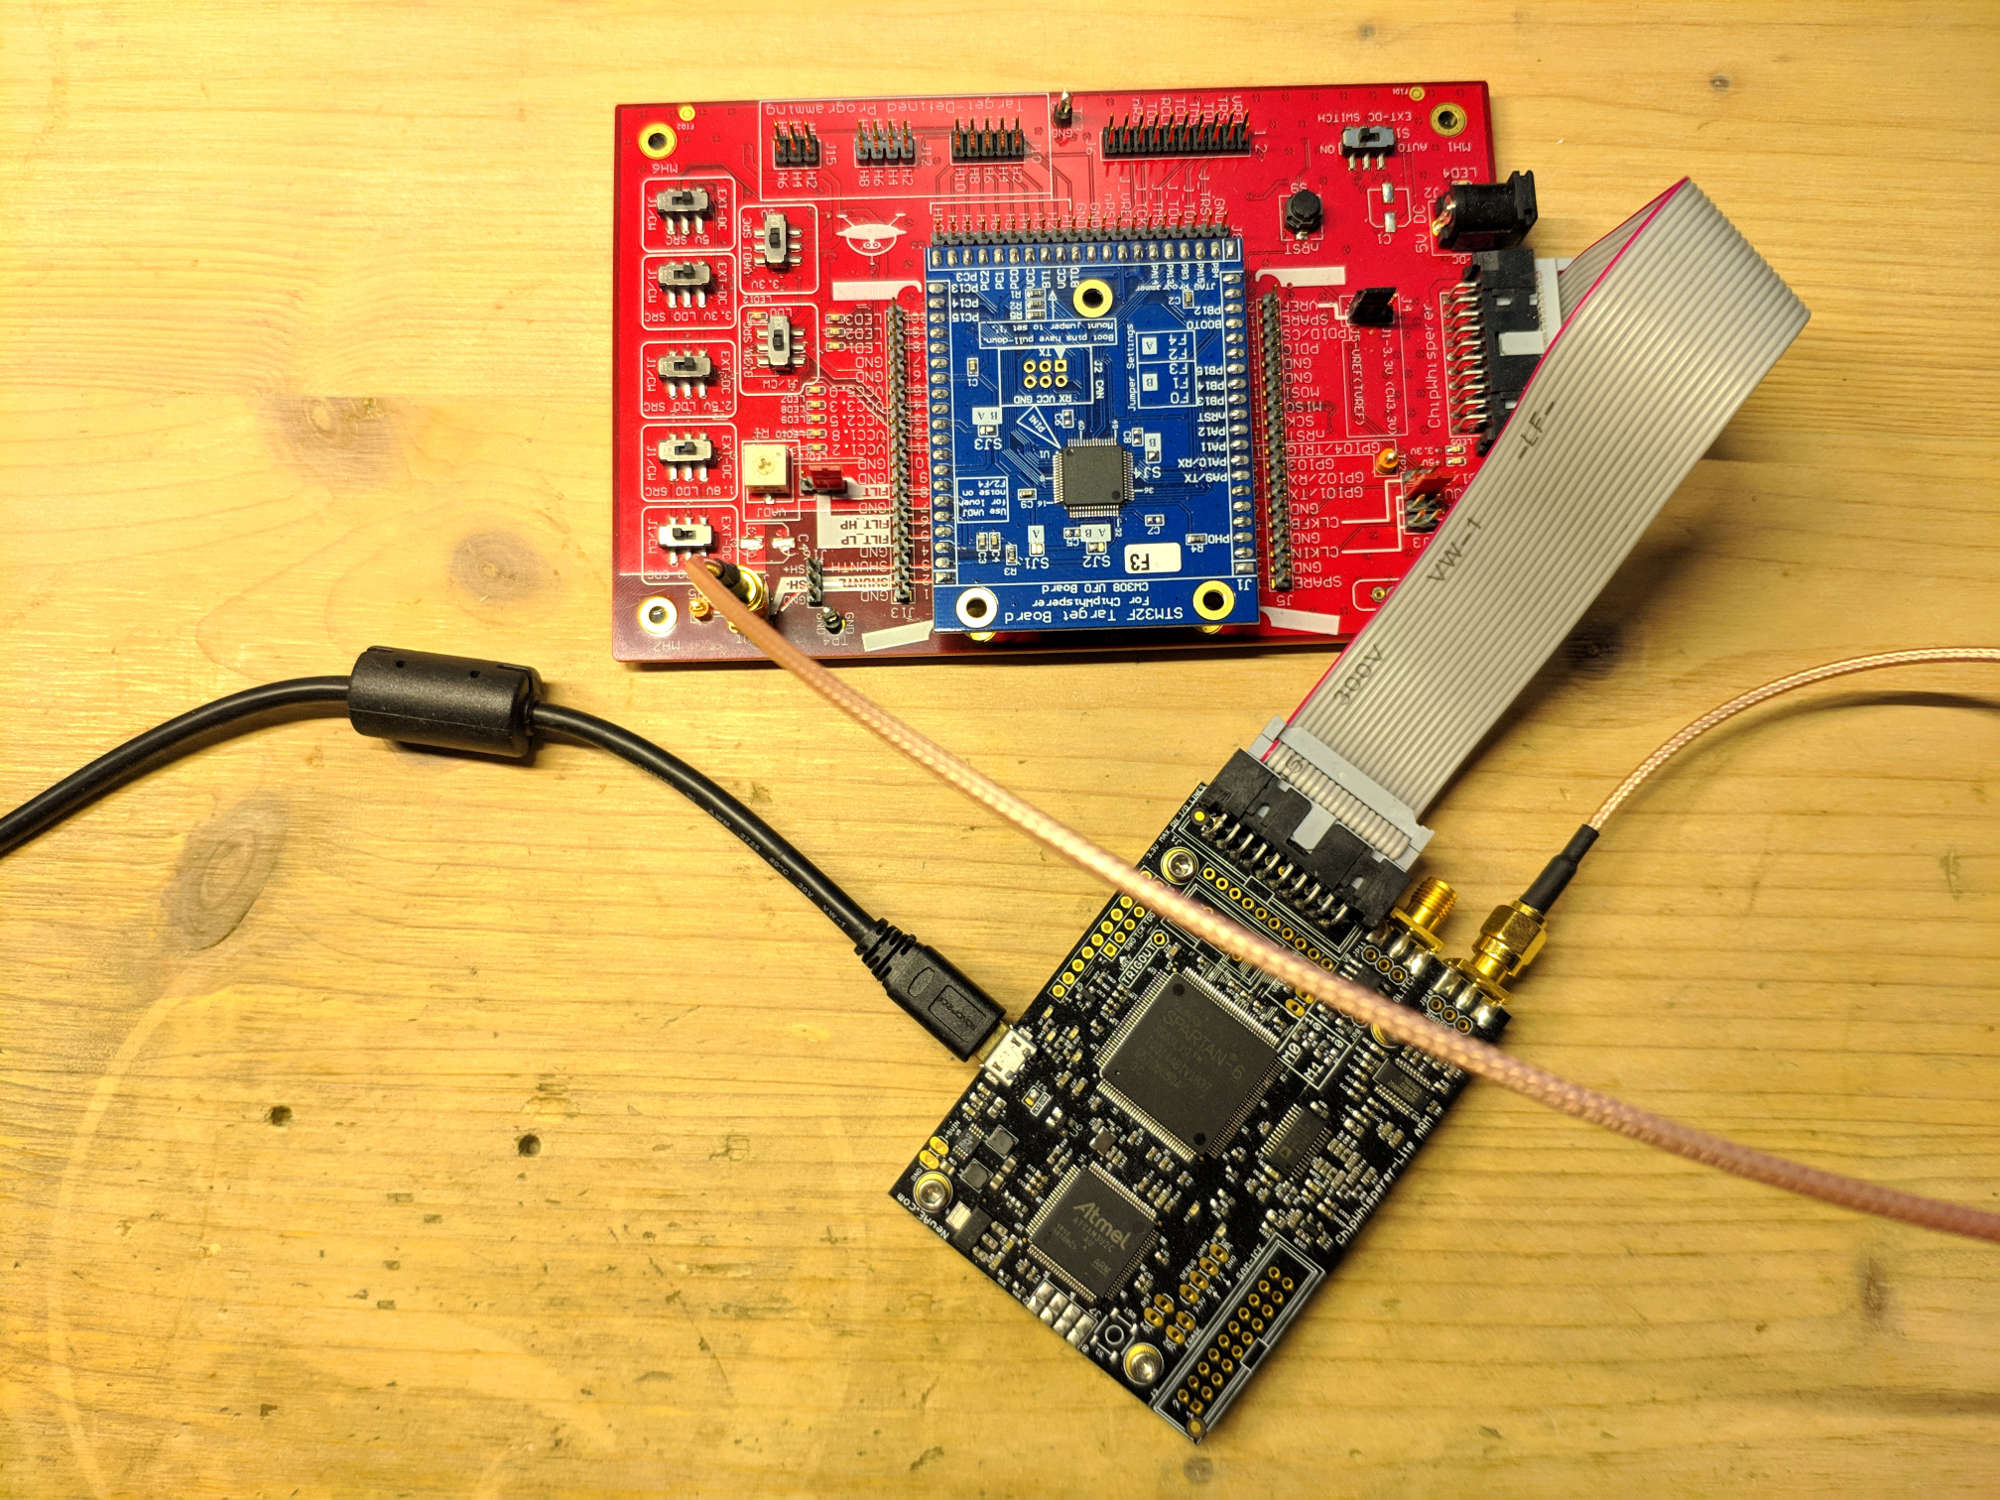
\includegraphics[width=0.8\linewidth]{img/hw_setup.jpg}

\end{frame}



\begin{frame}

    \frametitle{Traces aufzeichnen}


    \begin{itemize}
        \item mehrere ``Sätze'' an Aufzeichnungen erstellen
        \item mehrere Power-Traces pro Aufzeichnung
        \item verwendete Eingabedaten zusammen mit Power-Traces speichern
    \end{itemize}

\end{frame}



\begin{frame}

    \frametitle{Correlation Power Analysis}


    \begin{itemize}
        \item Zwischenwert abhängig von bekannten und unbekannten Parametern
        \item Modell für Stromverbrauch aus Zwischenwert $\rightarrow$
            Hamming-Gewicht
        \item Korrelationen für alle unbekannten Eingabedaten und alle Samples berechnen
        \item besten Kandidat auswählen
    \end{itemize}

\end{frame}



\begin{frame}

    \frametitle{Samples auswählen}


    \begin{itemize}
        \item auf Basis einer Analyse mit TVLA
        \item Angriff sonst nicht erfolgreich
        \item deutliche Verkürzung des zeitlichen Aufwands
    \end{itemize}

\end{frame}



\begin{frame}

    \frametitle{Test Vector Leakage Assessment (pro 32-bit Wort)}


    \centering
    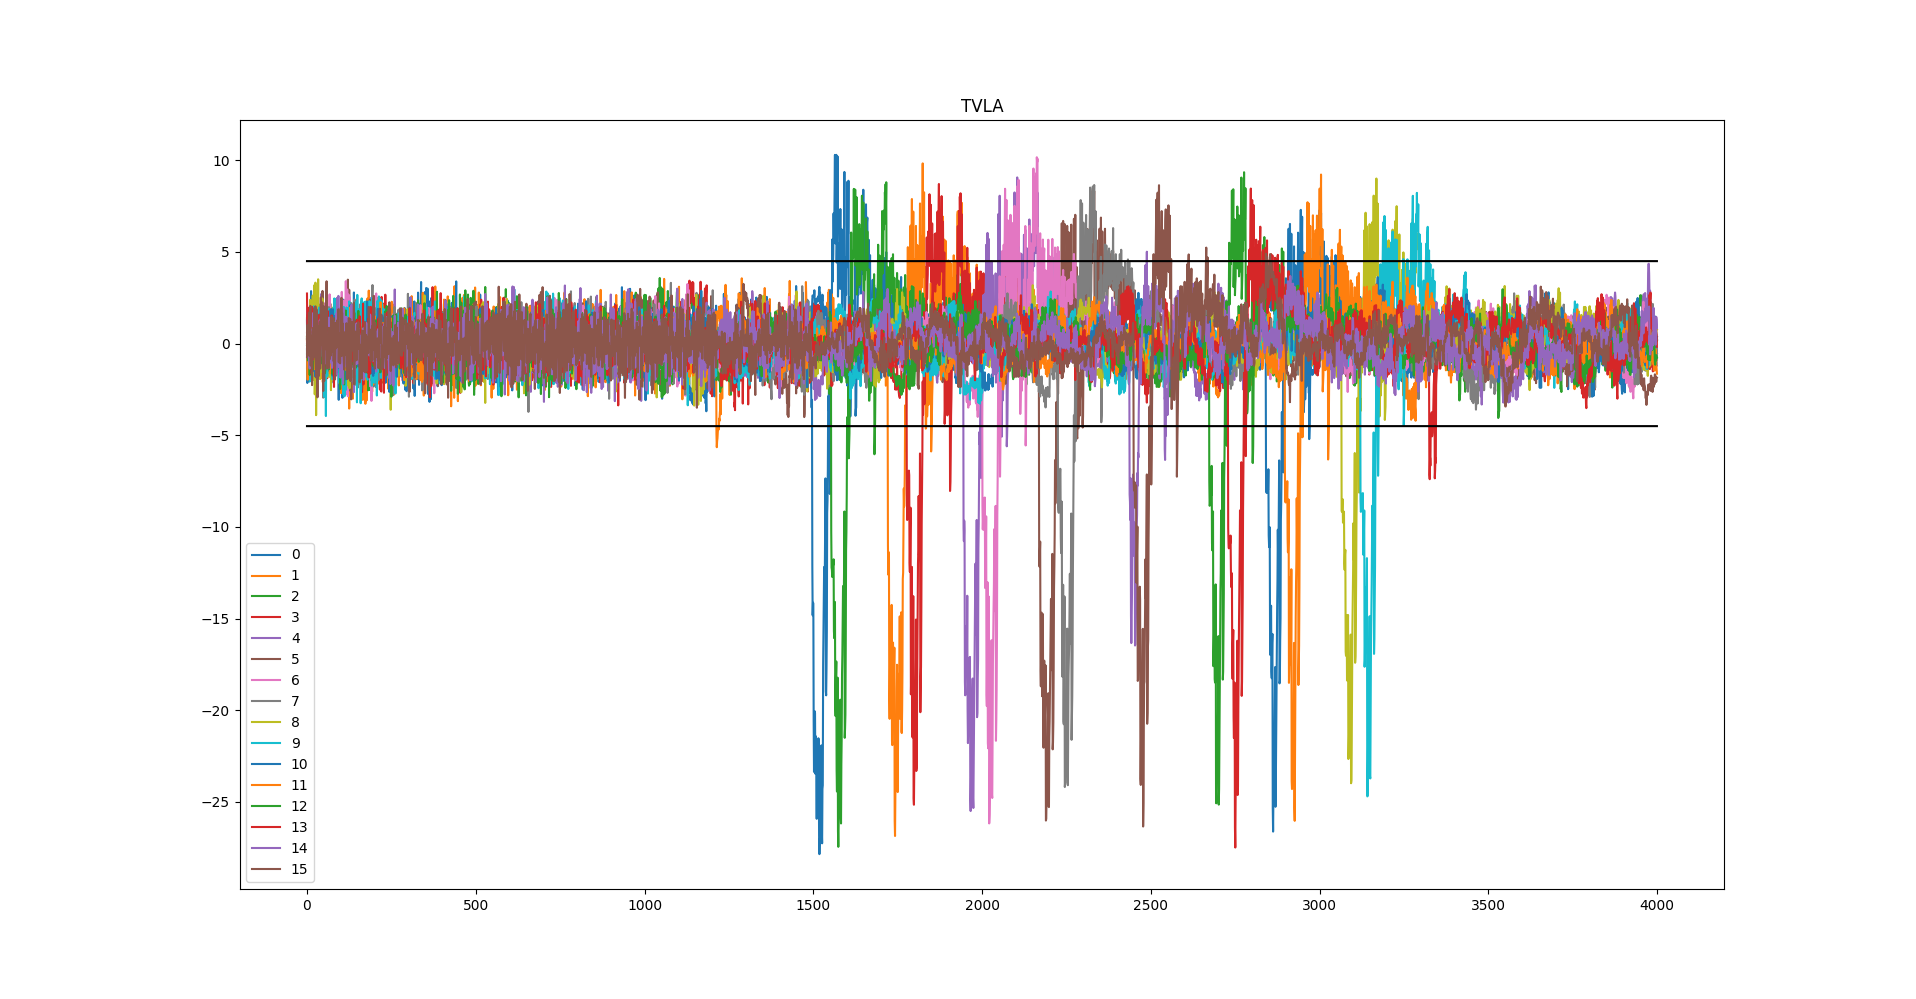
\includegraphics[width=\linewidth]{img/tvla_specific_overview.png}

\end{frame}



\begin{frame}

    \frametitle{Test Vector Leakage Assessment (pro Byte)}


    \centering
    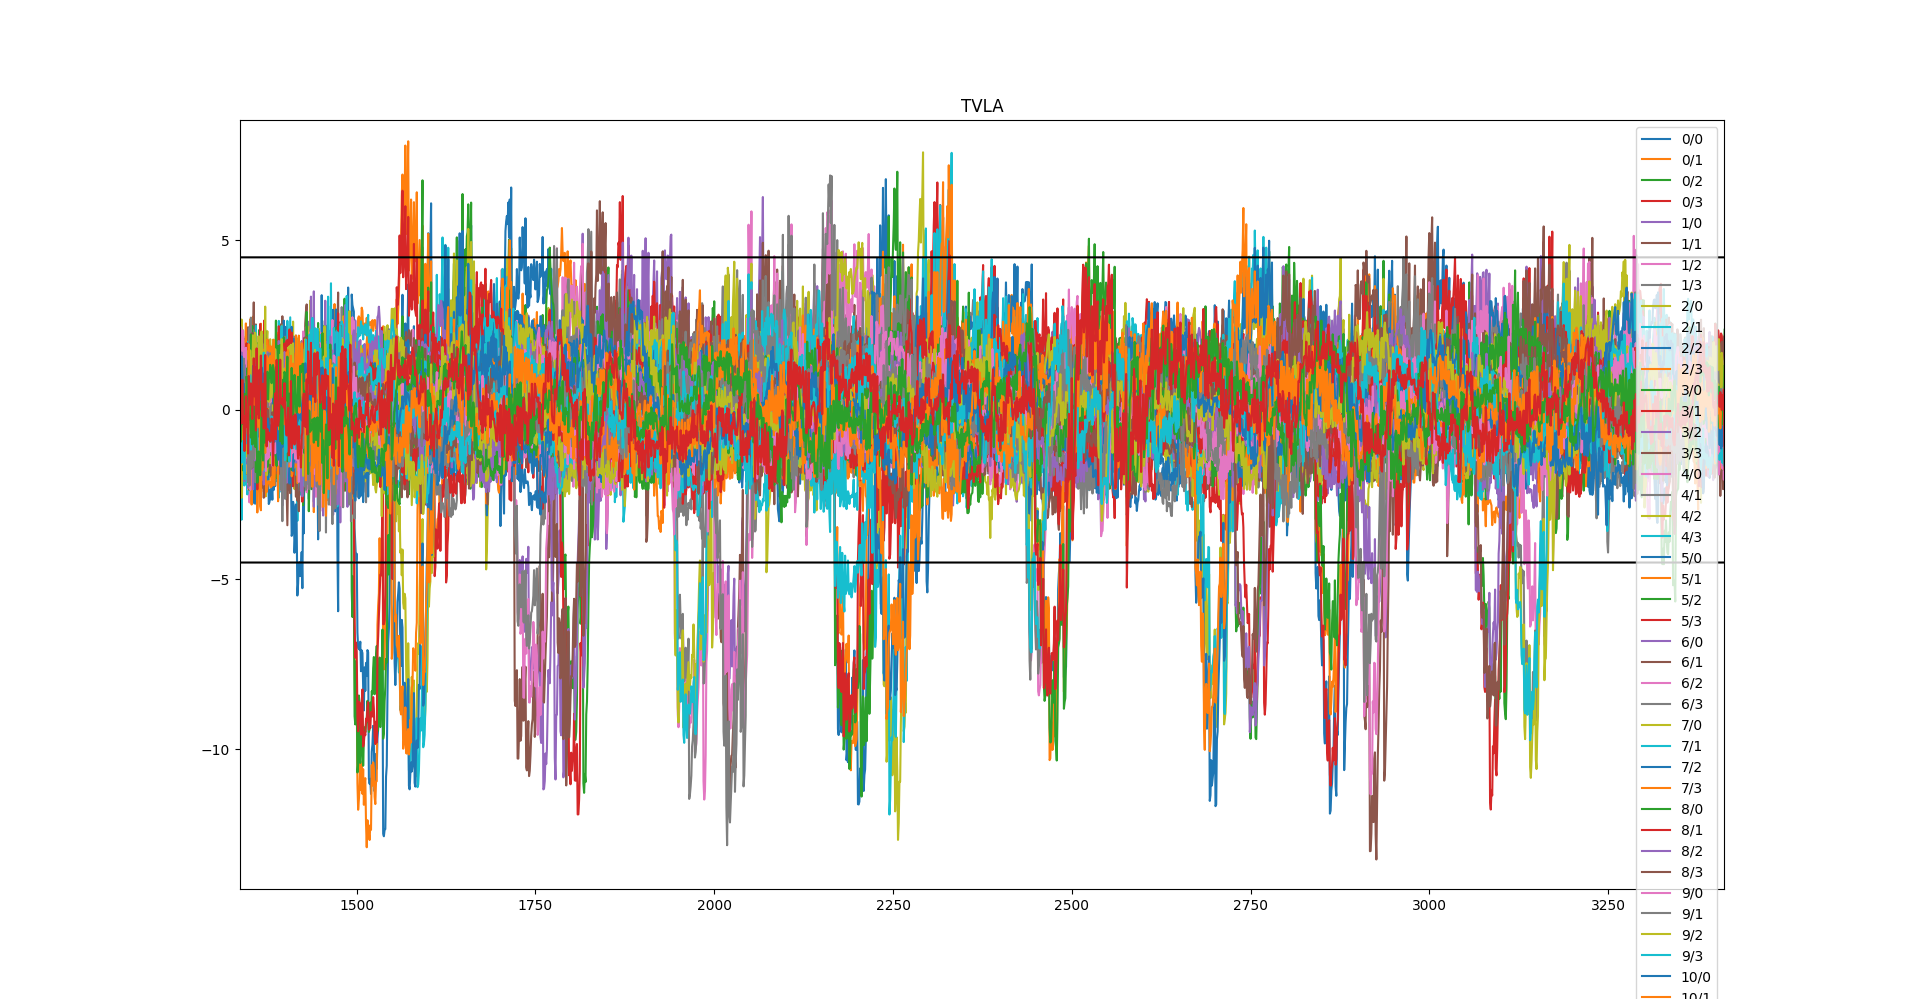
\includegraphics[width=\linewidth]{img/tvla_specific_bytes.png}

\end{frame}



\begin{frame}

    \frametitle{Normalized Inter-Class Variance (pro 32-bit Wort)}


    \centering
    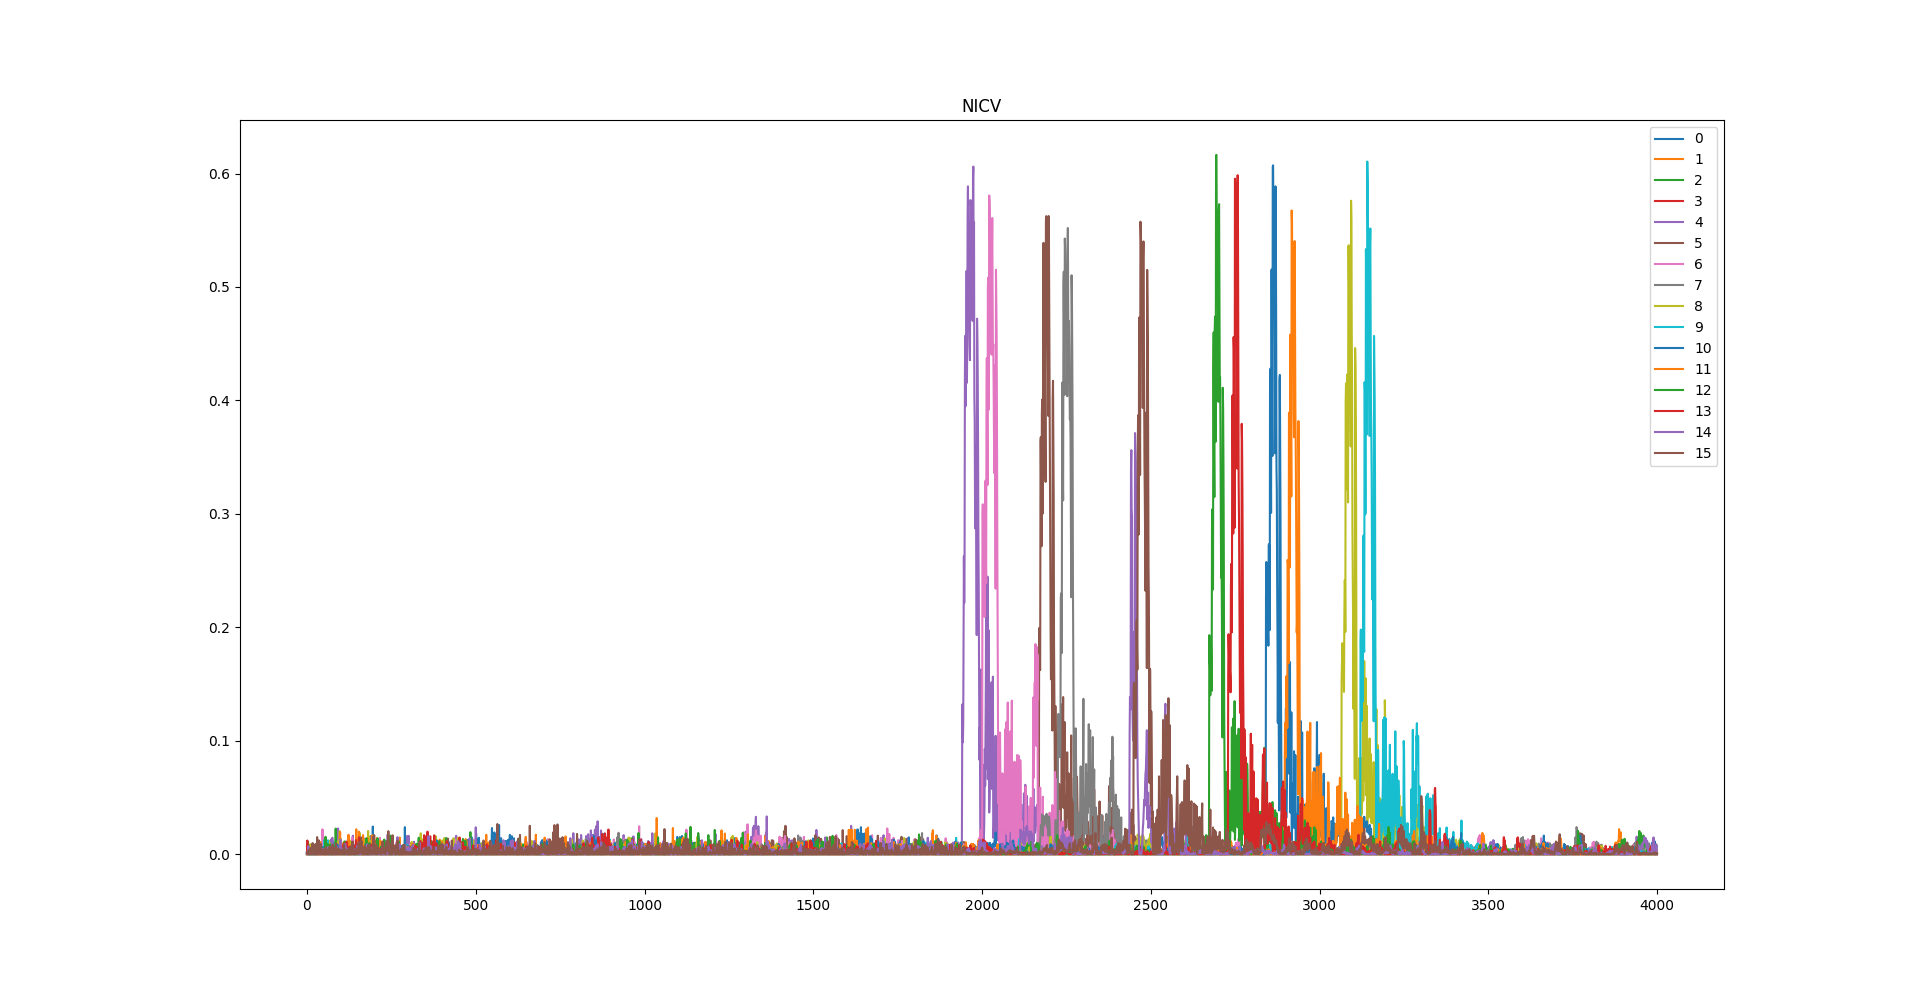
\includegraphics[width=\linewidth]{img/nicv_overview.png}

\end{frame}



\begin{frame}

    \frametitle{Variante 1: volle Kontrolle}


    \begin{itemize}
        \item zunächst erste Hälfte des Schlüssels angreifen
        \item Modell: HW(d1) = HW(d0 \^{} (a0 + b0))
        \item für k0: HW(d1) = HW(counter \^{} (C0 + k0))
        \item 32-bit Wort $\rightarrow$ divide-and-conquer $\rightarrow$ Byte
            für Byte beginnend beim LSB
        \item Ergebnis punktsymmetrisch $\rightarrow$ zwei Kandidaten mit
            gleicher absoluter Korrelation
    \end{itemize}

\end{frame}



\begin{frame}

    \frametitle{Variante 1: volle Kontrolle}


    \begin{itemize}
        \item anschließend die zweite Hälfte des Schlüssels angreifen
        \item Modell: HW(b1) = HW(b0 \^{} (c0 + ((d0 \^{} (a0 + b0))<<16)))
        \item für k4: HW(b1) = HW(k0 \^{} (k4 + ((counter \^{} (C0 + k0))<<16)))
        \item Ergebnis nicht symmetrisch $\rightarrow$ Auswahl des Schlüssels
            aus der ersten Hälfte möglich
    \end{itemize}

\end{frame}



\begin{frame}

    \frametitle{Variante 2: reduzierte Kontrolle}


    \begin{itemize}
        \item Counter und nonce0 bekannt, aber nicht beeinflussbar
        \item nonce1 und nonce2 beeinflussbar
        \item Traces mit zufälliger Eingabe, sowie nonce1 auf festen Wert
            fixiert aufzeichnen
    \end{itemize}

\end{frame}



\begin{frame}

    \frametitle{Variante 2: reduzierte Kontrolle}


    \begin{itemize}
        \item k2, k3, k6, k7 wie in Variante 1 angreifen
        \item Zwischenzustand nach der ersten Runde der beiden linken Spalten
            angreifen $\rightarrow$ teils auch Zwischenzustände in der
            quarterround
        \item mit der inversen quarterround den Initialzustand und damit k0, k1,
            k4, k5 berechnen
        \item ausgeführlich in der Dokumentation beschrieben
    \end{itemize}

\end{frame}



\section{Fazit}

\begin{frame}

    \frametitle{Probleme}


    \begin{itemize}
        \item Compiler-Optimierungen
        \item unklare/fehlerhafte Beschreibung im Paper
    \end{itemize}

\end{frame}



\begin{frame}

    \frametitle{Bewertung}


    \begin{itemize}
        \item Angriff auf ungeschütze Implementierung erfolgreich
        \item geschütze Implementierung möglicherweise mit erhöhtem Aufwand
            angreifbar
        \item bei beiden Varianten: Klar- und Schlüsseltext nicht benötigt
        \item Annahmen bei der zweiten Variante realistisch
        \item aufgrund immer weiterer Verbreitung (TLSv1.3) potentielles Risiko
    \end{itemize}

\end{frame}



\begin{frame}

    \frametitle{Fragen}


    Fragen? :)

\end{frame}




\end{document}

